\chapter{Pendahuluan}

\section{Latar Belakang}

Pada zaman industri ini, logistik merupakan suatu kebutuhan yang penting. Terdapat banyak perusahaan yang menawarkan jasa penyaluran dan penyimpanan barang.
Salah satunya adalah GOJEK yang memiliki sebuah business unit yang berfokus pada pengantaran barang yang dilakukan dengan menggunakan kendaraan truk.

Pada saat ini, dalam satu pesanan, perusahaan logistik tersebut melakukan sekali pengambilan (\textit{pickup}) dan pengantaran (\textit{drop off}) barang,
sehingga satu rute pengantaran hanya melayani sebuah pesanan. Untuk meningkatkan efisiensi pengantaran, sebuah rute pengantaran dapat melayani beberapa pesanan sekaligus.
Agar tercapainya efisiensi, diperlukan algoritma yang dapat menentukan rute terbaik dan tercepat.

Untuk penggambaran permasalahan, misalkan suatu graf tak berarah dengan $6$ buah simpul yang dilabeli dari $1$ sampai dengan $6$ dan $7$ buah sisi dengan berat tiap sisinya adalah $1$.
Sisi-sisi dari graf tersebut adalah $(1,2), (2,3), (1,4), (2,5), (3,6), (4,5), dan (5,6)$. Terdapat dua buah pesanan yang harus dilakukan. Pesanan ke-1 memiliki \textit{pickup},
yang disimbolkan dengan $P1$, terletak pada simpul $1$ dan drop off, yang disimbolkan dengan $D1$, terletak pada simpul $6$. Pesanan ke-2 memiliki \textit{pickup}, yang
disimbolkan dengan $P2$, terletak pada simpul $2$ dan \textit{drop off}, yang disimbolkan dengan $D2$, terletak pada simpul $3$.

\begin{figure}[H]
    \centering
    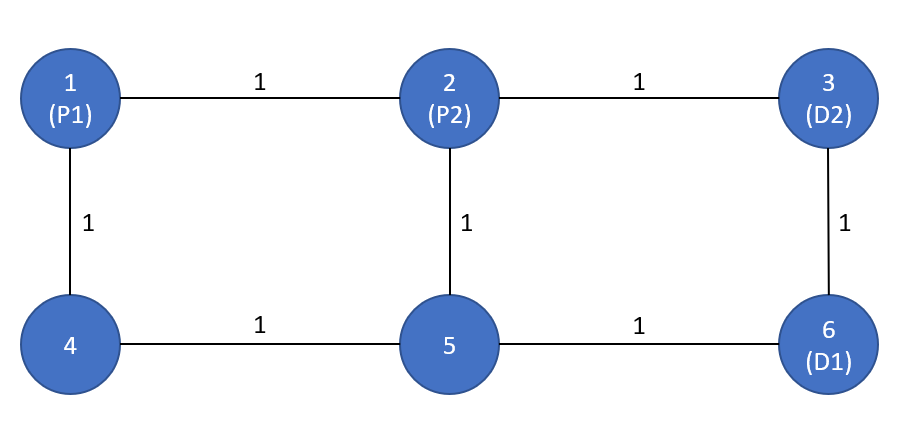
\includegraphics[width=1.0\textwidth]{resources/graph_init.png}
    \caption{Graf awal.}
\end{figure}

Pada umumnya kedua pesanan tersebut dilayani secara terpisah, contohnya pesanan satu memiliki rute $1-4-5-6$
yang memiliki \textit{cost} sebesar $3$ dan pesanan dua memiliki rute $2-3$ dengan \textit{cost} sebesar $1$.

\begin{figure}[H]
    \centering
    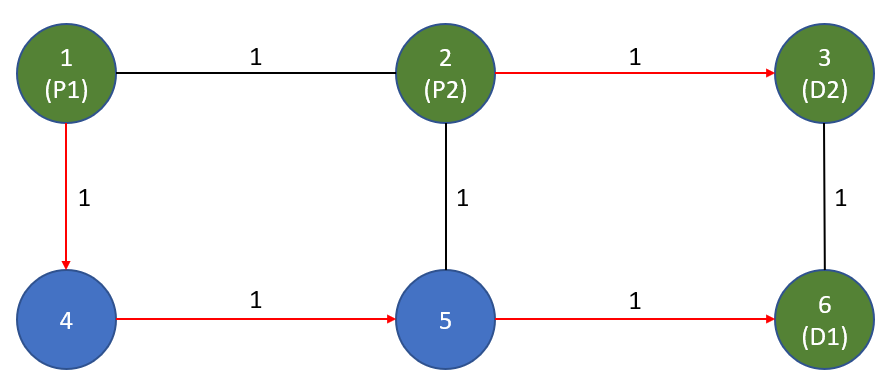
\includegraphics[width=1.0\textwidth]{resources/graph_routes.png}
    \caption{Graf yang memiliki rute 1-4-5-6 dan 2-3.}
\end{figure}

Namun, akan lebih efisien jika kedua pesanan tersebut dilakukan dalam sekali pengantaran, sehingga rute pengantarannya adalah $1-2-3-6$ dengan \textit{cost} sebesar $3$.
Pada saat berada simpul 1, truk melakukan \textit{pickup}, lalu truk menuju simpul 2, dan melakukan \textit{pickup} barang pesanan ke-2. Setelah itu, truk menuju simpul 3
dan menurunkan barang pesanan ke-2. Terakhir, truk menuju simpul 6  untuk melakukan \textit{drop off} pada barang pesanan ke-1.

\begin{figure}[H]
    \centering
    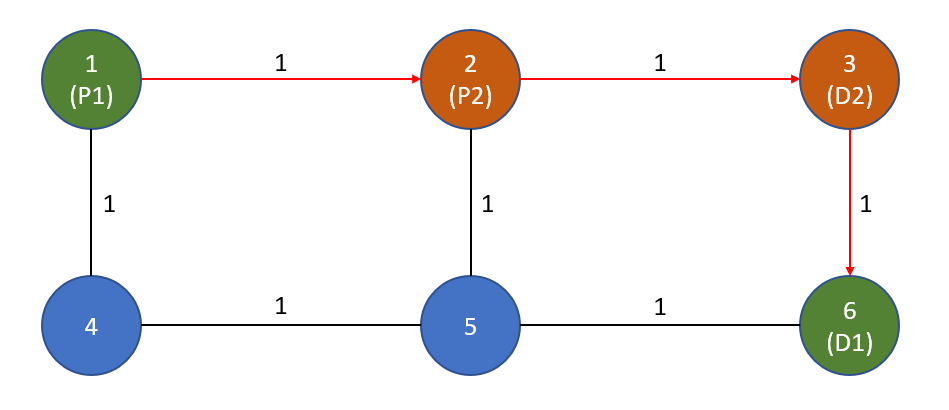
\includegraphics[width=1.0\textwidth]{resources/graph_optimal.png}
    \caption{Graf yang memiliki rute optimal 1-2-3-6.}
\end{figure}

\section{Rumusan Masalah}

Berdasarkan latar belakang pada subbab I.1, untuk menangani sebuah pesanan, dilakukan tepat 
sekali \textit{pickup} dan \textit{drop off}, namun telah ditunjukkan juga bahwa cara tersebut 
tidak selalu efisien dalam menangani banyak pesanan. 
Dari uraian tersebut, dapat dibentuk rumusan masalah sebagai berikut.

\begin{enumerate}
    % \item Bagaimana algoritma yang efisien untuk menentukan rute terbaik agar satu atau lebih pesanan dapat diselesaikan dalam sebuah rute pengantaran dengan sumber daya yang terbatas.
    \item Apa indikator pengukuran suatu rute pengantaran, sehingga dapat dibandingkan dengan rute pengantaran lainnya?
    \item Bagaimana cara untuk menentukan rute pengantaran yang efisien sehingga dapat menyelesaikan satau atau lebih pengantaran?
\end{enumerate}

\section{Tujuan}

Berikut adalah tujuan yang ingin dicapai dalam penulisan tugas akhir ini:

\begin{enumerate}
    \item Mengetahui indikator yang mengukur suatu rute pengantaran.
    \item Algoritma untuk menentukan rute terbaik agar satu atau lebih pesanan dapat diselesaikan dalam sebuah rute pengantaran dengan sumber daya yang terbatas.
\end{enumerate}

\section{Batasan Masalah}

Berikut adalah batasan-batasan masalah yang perlu diperhatikan:

\begin{enumerate}
    % \item Truk memiliki kapasitas maksimal, yang merupakan bilangan bulat positif.
    % \item Tiap pesanan memiliki cost bernilai bilangan bulat positif yang akan memakan kapasitas truk.
    % \item Penyimpanan truk bersifat LIFO atau last in first out.
    \item Selalu ada rute yang valid untuk setiap pesanan.
    \item Truk dapat melakukan \textit{drop off} suatu barang hanya setelah melakukan \textit{pickup}.
    % \item Truk dapat melakukan pengambilan barang dan pengiriman kapan saja.
    \item Daftar pickup dan \textit{drop off} sudah terdefinisi sebelum ditentukan rute truk.
\end{enumerate}

\section{Metodologi}

Berikut ini adalah tahapan dalam pengerjaan tugas akhir.

\begin{enumerate}
    \item Mendefinisikan permasalahan.\\
    Pada tahap ini, dilakukan pendefinisian dari permasalahan yang ada.
    \item Melakukan analisis terhadap permasalahan.\\
    Setelah mendapatkan definisi dari permasalahan, dilakukan analisis terhadap permasalahan, seperti masukan dan keluaran serta lingkup dan batasan permasalahan dan juga mempelajari algoritma shortest path untuk graf tak berarah.
    \item Mendesain algoritma.\\
    Pada tahap ini, dilakukan desain algoritma yang dapat menyelesaikan permasalahan dan memenuhi batasan-batasan masalah.
    \item Melakukan analisis algoritma.\\
    Terakhir, dilakukan analisis berupa kompleksitas algoritma dan kebenaran algoritma.
\end{enumerate}

\section{Jadwal Pelaksanaan Tugas Akhir}

Berikut adalah jadwal pengerjaan tugas akhir.

\begin{figure}[H]
    \centering
    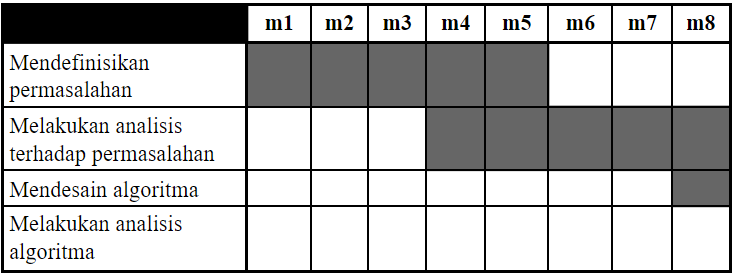
\includegraphics[width=1.0\textwidth]{resources/jadwa_pengerjaan.png}
    \caption{Jadwal pengerjaan tugas akhir.}
\end{figure}

Keterangan:
\begin{itemize}
    \item m1: 30 September 2019 - 6 Oktober 2019
    \item m2: 7 Oktober 2019 - 13 Oktober 2019
    \item m3: 14 Oktober 2019 - 20 Oktober 2019
    \item m4: 21 Oktober 2019 - 20 Oktober 2019
    \item m5: 28 Oktober 2019 - 3 November 2019
    \item m6: 4 November 2019 - 10 November 2019
    \item m7: 11 November 2019 - 17 November 2019
    \item m8: 18 November 2019 - 24 November 2019
\end{itemize}
